\documentclass[11pt,letterpaper]{article}
\usepackage[margin=1in,headheight=14pt]{geometry}
\usepackage[T1]{fontenc}
\usepackage{lmodern}
\usepackage{amsmath,amssymb,amsthm,mathtools}
\usepackage{microtype}
\usepackage{graphicx,booktabs,array,longtable}
\usepackage{xcolor}
\usepackage{enumitem}
\usepackage{fancyhdr}
\usepackage[unicode,colorlinks=true,linkcolor=navy,citecolor=navy,urlcolor=navy]{hyperref}
\definecolor{navy}{RGB}{24,49,75}
\definecolor{teal}{RGB}{0,112,115}
\hypersetup{pdftitle={Local Cauchy Laws and Infinite Transport of Dirichlet Zeros},
pdfauthor={Research report prepared for Vladimir Reshetnikov},
pdfsubject={Shrinking value intervals, positive Hermitian perturbations, electrical trace laws}}
\newtheorem{theorem}{Theorem}[section]
\newtheorem{lemma}[theorem]{Lemma}
\newtheorem{corollary}[theorem]{Corollary}
\newtheorem{proposition}[theorem]{Proposition}
\theoremstyle{remark}
\newtheorem{remark}[theorem]{Remark}
\numberwithin{equation}{section}
\setlist{itemsep=3pt,topsep=5pt}
\setlength{\parskip}{3pt}
\setlength{\emergencystretch}{2em}
\pagestyle{fancy}
\fancyhf{}
\fancyhead[L]{\small\sffamily Dirichlet zeros: local laws and transport}
\fancyhead[R]{\small\sffamily Research report}
\fancyfoot[C]{\small\thepage}
\renewcommand{\headrulewidth}{0.3pt}
\begin{document}
\begin{titlepage}
\vspace*{0.7in}
{\color{teal}\sffamily\large MATHEMATICAL RESEARCH\par}
\vspace{0.2in}
{\color{navy}\huge\bfseries Local Cauchy Laws and\par
Infinite Transport of\par Dirichlet Zeros\par}
\vspace{0.25in}
{\Large Arbitrarily shrinking value windows, Hermitian perturbations,\par
and electrical trace asymptotics\par}
\vspace{0.35in}
{\large Prepared for Vladimir Reshetnikov\par}
{November 26, 2026\par}
\vspace{0.35in}
\begin{abstract}
Starting from the proved zero-location theorem for Dirichlet $L$-functions
and an earlier graph-coupled-zero construction, we derive three related
extensions.  First, if $F$ is a phase-real completed primitive Dirichlet
function and $t$ is uniform on $[T,2T]$, the normalized logarithmic
derivative $2F'(t)/(F(t)\log T)$ satisfies a local Cauchy law for every
moving interval shrinking to a finite point, with no lower bound on its
width.  Second, for Hermitian $A$ and $B\succeq0$, the canonical zero
transport density of $\det(\operatorname{diag}(F_i)A+
\operatorname{diag}(F_i'))$ obeys
$(\log T)\sigma(Tu)du\to(2\operatorname{tr}B/\pi)du$.
We give an exact Poisson regularization and every term of its logarithmic
asymptotic expansion.  Third, a squared-ordinate construction has
accumulated transport asymptotic to
$\Delta K\sqrt X\log X/(4\pi n)$, where $\Delta K$ is the decrease in the
network's Kirchhoff index.  All multiplicities and shared zeros are
allowed.  Complete proofs, source provenance, exact algebraic checks,
and reproducible numerical diagnostics accompany the report.
\end{abstract}
\vfill
{\small\color{navy}Proof status: complete human-readable arguments;
not Lean-formalized.  Novelty status: compared with the specified sources
and targeted primary literature; historical priority remains subject to
further scholarly review.}
\end{titlepage}

\tableofcontents
\newpage
\section*{Main result at a glance}
\addcontentsline{toc}{section}{Main result at a glance}

Write $\Xi(t)=\xi(1/2+it)$ for the real Riemann xi-function on the
critical line.  One particularly concrete consequence proved here is
\begin{equation*}
 \left|\left\{t\in[T,2T]:
        \left|\frac{\Xi'(t)}{\Xi(t)}\right|<e^{-T}\right\}\right|
       \sim\frac{4Te^{-T}}{\pi\log T}.
\end{equation*}
Although the tested derivative window shrinks exponentially, its total
preimage length has an exact leading constant.  This is a continuous
measure statement, not a claim about what a finite sampling grid sees.
Theorem~\ref{thm:local-cauchy} proves the general result for all primitive
Dirichlet completions and all shrinking windows centered at a finite
normalized value.

The same positive analytic phase measures movement of zeros when a
Hermitian coupling is increased.  Adding a graph edge of conductance $h$
produces total movement, clipped to $[-T,T]$, of
\[
 \frac{8h}{\pi}\frac{T}{\log T}(1+o(1)).
\]
The total over the entire real line is therefore infinite.  Its Poisson
regularization is exactly computable from a finite determinant, and its
full expansion records the conductors and the graph.

For the separate construction using squared ordinates, strengthening the
graph changes the leading coefficient to an electrical invariant:
\[
 \frac{K(G_0)-K(G_1)}{4\pi n}\sqrt X\log X,
 \qquad K(G)=\sum_{a<b}R_{ab}(G).
\]
This supplies an infinite resistance analogue with a proved convergence
and Tauberian argument.  The two coordinate choices define different
entire functions and are kept distinct throughout.

\section{Source review and the precise new contribution}
\label{sec:sources}

\subsection{What was taken from the three requested sources}

The upstream repository was inspected at commit
\texttt{72fead102f663d5c7a407964a13dc0cf9d977207}.  Its
\texttt{grh-compact/src/Statements.lean} imports Mathlib and defines the
zero-location statements, while \texttt{src/Main.lean} proves those
statements and Mathlib's \texttt{RiemannHypothesis}.  The scope is the
Riemann zeta function and \emph{Dirichlet} $L$-functions, including all
positive moduli and imprimitive characters.  It does not state GRH for
arbitrary Artin or automorphic $L$-functions~\cite{upstream}.

The repository reports successful compilation, kernel replay, and
Comparator checks, with the five main theorems depending only on
\texttt{propext}, \texttt{Classical.choice}, and \texttt{Quot.sound}.
The readable and compact editions contain roughly 300,000 and 76,000
lines respectively.  The pinned source and selected central files were
read for this report; the complete build was not replayed here.
Andrew Sutherland's verification page records independent checks of this
same shorter release~\cite{sutherland}.  The requested Wikipedia page
reports the November 2026 proof and its verification~\cite{wikipedia};
the exact formal statements, rather than the encyclopedia's broad
terminology, determine the scope used below.

The source's central new argument is an \emph{arithmetic covolume
comparison}, not the spectral construction in this report.  In the
compact edition, \texttt{New/Endgame/ShortAndEnough.lean} supplies many
small integral forms and an almost-spanning dimension bound;
\texttt{LongForms.lean} supplies a lower bound for the same integral
covolume using heights and the product formula.  In the notation of
\texttt{New/Main.lean}, cancellation of the main height leads to
\[
 mR\le (\log b)^2\,\mathrm{budget},\qquad m\asymp\sqrt x,
\]
where $R$ is a smoothed prime-power remainder.  The compact
\texttt{OneSidedCriterion.lean} then applies a one-sided Landau argument;
functional equations complete the zero-location conclusion.
The useful conceptual pattern is to retain positivity and a common
determinant while comparing two descriptions of it.  Our argument
uses that pattern in a new analytic construction after importing the
proved zero-location statement.

The ProveIt tree was inspected at commit
\texttt{041d8032541746f2ac2e686fbe437f8092771670}.  Its README distinguishes
61 imported older research packets from independent checking and states
that their Lean excerpts are not part of its root Lake package
\cite{proveit}.  The review here read the index, relevant merged-article
sections, the graph packet, the robust-spectrum packet, and descriptions
and targeted source searches in seven later incoming packets.  It is
not a proof audit of every report in the collection.  Retrieved archive
bytes were checked against their pinned Git blob identifiers, and a
source manifest is included with this report.

\subsection{The immediate predecessor}

The packet \texttt{graph\_coupled\_zeros\_2026-11-26.zip} already proves
the finite polynomial identity
\[
 P_G(z)=\det\!\left(\operatorname{diag}(p_i(z))L_G+
                             \operatorname{diag}(p_i'(z))\right)
\]
has real zeros, with a compression interpretation and an exact total
displacement expressed through effective resistances.  It also proves
real-zero preservation, collision multiplicities, and bounded zero-count
discrepancy for entire inputs~\cite{priorgraph}.  Those facts are prior
work; the essential half-plane argument is reproduced below for a
self-contained proof of the extensions.

Its final section explicitly asks whether one can regularize the
displacement of \emph{all} completed Dirichlet zeros and obtain an
infinite analogue of the electrical formula.  Theorems
\ref{ut:exact}--\ref{ut:expansion} answer the convergence and asymptotic
part for the original construction.  Theorem~\ref{thm:electrical-infinite}
gives an electrical counterpart for a separately defined squared-ordinate
construction.  In particular, an unweighted infinite sum is generally
\emph{divergent}; its precise growth and convergent transforms are the
correct objects.

\subsection{Novelty compared with primary literature}

The mathematical components have clear precedents.  Matrix meromorphic
Herglotz theory already provides higher-order interlacing
\cite{reiffenstein}.  Spectral-shift logarithms and trace identities are
classical~\cite{bgn}.  Herglotz boundary distributions and Cauchy laws are
treated by Aizenman and Warzel~\cite{aizenmanwarzel}.  Sodin proves a weak
Cauchy limit for the normalized logarithmic derivative under RH
\cite[Section 3.4.5, equation (55)]{sodin}; Najnudel and Nikeghbali develop
that theme further~\cite{najnudel}.  Differencing and derivative
deformations of completed $L$-functions also predate this work
\cite{lagarias,farmergonek}.

The contributions developed and proved here are the following:
\begin{enumerate}
\item An arithmetic local limit for the logarithmic derivative valid for
\emph{arbitrarily shrinking moving value intervals}, including relative
asymptotics for exponentially small widths
(Theorem~\ref{thm:local-cauchy}).
\item A universal local transport limit for positive Hermitian
perturbations of completed Dirichlet determinants, on every fixed
macroscopic real window (Theorem~\ref{ut:main}).
\item An all-orders Poisson-smoothed expansion whose coefficients are
explicit finite matrix traces, separating the first conductor and graph
corrections (Theorem~\ref{ut:expansion}).
\item A squared-ordinate transport law with exact coefficient given by
the decrease in the graph's Kirchhoff index
(Theorem~\ref{thm:electrical-infinite}).
\end{enumerate}
No identical statement was located in the inspected ProveIt material or
the targeted primary-literature search.  This is a documented novelty
comparison, not certification of worldwide publication priority.  The
proofs below establish the claims as mathematical statements independently
of that priority question.

\paragraph{Dependence on RH/GRH.}
The given zero-location theorem makes the relevant logarithmic derivatives
have a strict half-plane sign.  The functional equation and gamma-factor
asymptotics then determine the constants.  No simplicity of zeros,
linear independence of ordinates, pair-correlation conjecture, or
identification of the new determinants with Euler products is assumed.
The proofs are written out in ordinary mathematics.  They have not been
formalized in Lean in this packet.

% Standalone mathematical section. Requires amsmath,amssymb,amsthm.
% Uses theorem, lemma, corollary, proposition, remark environments.
% Citation keys, if added by parent: BGN2018, Reiffenstein2022, DLMF.
\section{A universal law for the displacement of infinitely many zeros}
\label{sec:universal-transport}

This section supplies the convergence and regularization missing from the
earlier graph-coupled-zero construction. The basic spectral-shift mechanism
is classical; see \cite{bgn,reiffenstein}. The contribution developed here is its arithmetic asymptotic:
the total zero displacement has an explicit universal leading coefficient,
and every coefficient of its Poisson-smoothed expansion is a finite matrix
trace. No simplicity, zero-spacing, linear-independence, or pair-correlation
assumption is used.

\subsection{Inputs and a canonical measure of displacement}
\label{sec:setup}

Let $F_1,\ldots,F_n$ be phase-real primitive completed Dirichlet functions,
allowing repetitions and the pole-removed zeta completion. Thus, for a
primitive nonprincipal character $\chi$ of conductor $q$ and parity $a$,
\[
 \Lambda_\chi(s)=(q/\pi)^{(s+a)/2}\Gamma((s+a)/2)L(s,\chi),
 \qquad F_\chi(z)=\eta_\chi^{-1}\Lambda_\chi(1/2+iz),
 \qquad \eta_\chi^2=\varepsilon_\chi.
\]
For zeta set $q=1$ and
\[
 F_\zeta(z)=\xi(1/2+iz),\qquad
 \xi(s)=\tfrac12s(s-1)\pi^{-s/2}\Gamma(s/2)\zeta(s).
\]
The functional equation makes each $F_i$ real entire, including for complex
characters. Invoke the Dirichlet zero-location theorem to conclude that
all its zeros are real. Its order-one canonical product gives, off those
zeros,
\[
 g_i(z)=\frac{F_i'(z)}{F_i(z)},\qquad
 \operatorname{Im}g_i(z)<0\quad(\operatorname{Im}z>0).
\]
Indeed, with zeros listed with multiplicity,
\[
 \operatorname{Im}g_i(x+iy)
   =-y\sum_{\rho\in\mathcal Z(F_i)}\frac1{|x+iy-\rho|^2}<0.
\]
The real constant from the canonical product does not affect this formula;
the series converges locally uniformly away from the zeros.

For a fixed Hermitian $n\times n$ matrix $A$, define
\begin{align}
 P_A(z)&=\det\!\left(\operatorname{diag}(F_i(z))A+
                           \operatorname{diag}(F_i'(z))\right),
             \label{ut:defPA}\\
 M_A(z)&=A+\operatorname{diag}(g_i(z)). \label{ut:defMA}
\end{align}
The first expression is entire and real: its principal-minor expansion
has real coefficients multiplying products of real entire functions.
Away from the input zeros,
$P_A=(\prod_iF_i)\det M_A$. Since $\operatorname{Im}M_A\prec0$ in the
upper half-plane, $M_A$ is invertible there. Consequently $P_A$ is nonzero
and all its zeros are real.

Fix $0\ne B\succeq0$ Hermitian, of rank $r$, and set $A_1=A+B$.
At real $x$ avoiding all input and output zeros, define
\begin{equation}\label{ut:defshift}
 \sigma_{A,B}(x)=n_+(M_{A+B}(x))-n_+(M_A(x)).
\end{equation}
Values on the excluded discrete set are immaterial for integration.
Here $n_+$ counts strictly positive eigenvalues with multiplicity.
Since $B\succeq0$ and has rank $r$,
\begin{equation}\label{ut:shiftbound}
       0\leq\sigma_{A,B}(x)\leq r.
\end{equation}
This is the canonical rightward zero-crossing count. In particular, it
avoids the ambiguous subtraction of two infinite zero-counting functions.

\begin{theorem}[Exact displacement measure and trace identity]
\label{ut:exact}
There is a holomorphic logarithm $\mathcal L_{A,B}$ on the upper
half-plane satisfying
\[
 e^{\mathcal L_{A,B}(z)}=\frac{P_{A+B}(z)}{P_A(z)},\qquad
 0<\operatorname{Im}\mathcal L_{A,B}(z)<r\pi,
 \qquad \mathcal L_{A,B}(iy)\longrightarrow0\quad(y\to\infty).
\]
Its boundary imaginary part is $\pi\sigma_{A,B}$ almost everywhere, and
\begin{equation}\label{ut:poisson}
 \boxed{\quad
 \int_{\mathbb R}\frac{y^2\sigma_{A,B}(t)}{t^2+y^2}\,dt
       =y\operatorname{Im}\mathcal L_{A,B}(iy)
       \quad(y>0).\quad}
\end{equation}
More generally,
\begin{equation}\label{ut:poisson-general}
 \operatorname{Im}\mathcal L_{A,B}(x+iy)
     =\int_{\mathbb R}\frac{y\sigma_{A,B}(t)}{(t-x)^2+y^2}\,dt.
\end{equation}
Writing $\nu_A$ for the locally finite zero-counting measure of $P_A$,
including multiplicity, one has the distributional equality
\begin{equation}\label{ut:distribution}
         d\sigma_{A,B}=d\nu_A-d\nu_{A+B}.
\end{equation}
Consequently every $\varphi\in C_c^1(\mathbb R)$ satisfies the exact,
finite identity
\begin{equation}\label{ut:testtrace}
 \sum_{P_{A+B}(\beta)=0}\!\operatorname{ord}_\beta(P_{A+B})\varphi(\beta)
 -\sum_{P_A(\alpha)=0}\!\operatorname{ord}_\alpha(P_A)\varphi(\alpha)
   =\int_{\mathbb R}\varphi'(t)\sigma_{A,B}(t)\,dt.
\end{equation}
Common zeros cancel with their exact multiplicities.
\end{theorem}

\begin{proof}
Write $B=VV^*$ with $V$ an $n\times r$ matrix of full column rank. Set
\[
 H(z)=V^*M_A(z)^{-1}V.
\]
For every invertible matrix $M$,
\[
 \operatorname{Im}(M^{-1})
       =-M^{-*}(\operatorname{Im}M)M^{-1}.
\]
Thus $\operatorname{Im}H(z)\succ0$ in the upper half-plane. The eigenvalues
of $I_r+H(z)$ all lie in that half-plane, so its principal matrix logarithm
is holomorphic. Put
\[
 \mathcal L_{A,B}(z)=\operatorname{tr}\log(I_r+H(z)).
\]
The sum of the principal arguments of its $r$ eigenvalues lies strictly
between $0$ and $r\pi$. The determinant lemma gives
$e^{\mathcal L_{A,B}}=\det M_{A+B}/\det M_A=P_{A+B}/P_A$.
The asymptotic lemma below gives $H(iy)=O(1/\log y)$ and hence the asserted
normalization at infinity.

At a real regular point $x$, the matrices $M_A(x)$ and $H(x)$ are Hermitian.
Approach from the upper half-plane. Each negative eigenvalue of $I+H(x)$
has limiting argument $\pi$ and each positive eigenvalue has limiting
argument zero. Therefore
\[
 \pi^{-1}\operatorname{Im}\mathcal L_{A,B}(x+i0)=n_-(I_r+H(x)).
\]
To identify this with \eqref{ut:defshift}, take the inertia of
\[
 \begin{pmatrix}M_A(x)&V\\ V^*&-I_r\end{pmatrix}
\]
using its two Schur complements. They give, respectively,
$n_+(M_A(x))+n_-(I_r+H(x))$ and $n_+(M_A(x)+B)$.
This proves the boundary formula.

The imaginary part of $\mathcal L_{A,B}$ is a bounded harmonic function
on the upper half-plane. The Poisson representation for bounded harmonic
functions gives \eqref{ut:poisson-general}. There is no additional linear
term or singular boundary measure: bounded harmonic functions are the
Poisson extensions of their bounded almost-everywhere boundary values.
This proves \eqref{ut:poisson} as well; its integral is absolutely finite
by \eqref{ut:shiftbound}.

For completeness, multiplicities in \eqref{ut:distribution} can be read
directly from the entire quotient, without a simplicity assumption.
At a real $x_0$, locally write
\[
 \frac{P_{A+B}(z)}{P_A(z)}=(z-x_0)^k a(z),\qquad
 k=\operatorname{ord}_{x_0}P_{A+B}-\operatorname{ord}_{x_0}P_A,
\]
with $a$ analytic, real and nonzero near $x_0$. The boundary argument
of $\log(z-x_0)$ drops by $\pi$ when crossing $x_0$ from left to right.
Hence $\sigma_{A,B}$ jumps by $-k$. Away from this discrete divisor it
is locally constant. These are precisely the atoms of
$\nu_A-\nu_{A+B}$. Integration by parts gives \eqref{ut:testtrace}.
\end{proof}

\begin{remark}[Why this measures motion rather than just a count]
For a rank-one addition, $1+H(z)$ is a scalar meromorphic function with
positive imaginary part. Its real poles and zeros interlace after common
factors are canceled. The set where its boundary value is negative is a
disjoint union of intervals from an old zero to the following new zero;
$\sigma_{A,B}$ is their indicator. Thus its integral over a window is
the total length of the moving-zero intervals clipped to that window.
For general $B$, decompose it into $r$ positive rank-one terms and apply
this observation successively. The crossing counts add and telescope
to \eqref{ut:defshift}, so their total is independent of this decomposition.
No separately divergent sum $\sum\beta-\sum\alpha$ is used.
\end{remark}

\subsection{Arithmetic input at large complex arguments}

Put
\begin{equation}\label{ut:conductorconstants}
 c_i=\tfrac12\log\!\left(\frac{q_i}{2\pi}\right),\qquad
 C=\operatorname{diag}(c_1,\ldots,c_n),\qquad
 \ell_y=\tfrac12\log y.
\end{equation}

\begin{lemma}[Uniform radial logarithmic derivative]\label{ut:radial}
For every compact subset $K$ of the upper half-plane,
\begin{equation}\label{ut:radial-asymptotic}
 g_i(Tz)=-i\left(\tfrac12\log T+c_i+\tfrac12\log(-iz)\right)
                    +O_K(T^{-1})\qquad(z\in K).
\end{equation}
The logarithm is the principal one; $-iz$ is in the right half-plane.
In particular
\begin{equation}\label{ut:imag-asymptotic}
 g_i(iy)=-i(\ell_y+c_i)+O(y^{-1}).
\end{equation}
All conductors, characters, and matrices are fixed as $T$ or $y$ tends
to infinity.
\end{lemma}

\begin{proof}
For a primitive nonprincipal character the functional equation gives
\[
 g_i(Tz)=-i\frac{\Lambda_{\overline\chi}'(1/2-iTz)}
                         {\Lambda_{\overline\chi}(1/2-iTz)}.
\]
Write $s=1/2-iTz$. Uniformly for $z\in K$, $\operatorname{Re}s$ tends
linearly to $+\infty$ and $s$ stays in a closed subsector of the right
half-plane. Logarithmic differentiation of the completion gives
\[
 \frac{\Lambda_{\overline\chi}'(s)}{\Lambda_{\overline\chi}(s)}
 =\tfrac12\log(q_i/\pi)
       +\tfrac12\psi((s+a_i)/2)
       +\frac{L'(s,\overline\chi)}{L(s,\overline\chi)}.
\]
The functional equation and completion are standard \cite{dlmfdirichlet}.
The absolutely convergent Euler-product logarithmic derivative is
exponentially small in $\operatorname{Re}s$. The uniform Stirling
expansion $\psi(w)=\log w+O(|w|^{-1})$ gives
\[
 \tfrac12\log T+c_i+\tfrac12\log(-iz)+O_K(T^{-1}).
\]
For zeta, logarithmic differentiation of the pole-removing factor adds
$1/s+1/(s-1)=O_K(T^{-1})$, so the same formula holds with $q_i=1$.
\end{proof}

\subsection{The macroscopic transport law}

\begin{theorem}[Universal macroscopic zero transport]\label{ut:main}
With the preceding fixed inputs, matrices, and $0\ne B\succeq0$, the
positive measures
\begin{equation}\label{ut:weaklimit}
   (\log T)\sigma_{A,B}(Tu)\,du
        \ \longrightarrow\ \frac{2\operatorname{tr}B}{\pi}\,du
        \qquad(T\to\infty)
\end{equation}
converge against every continuous compactly supported test function on
$\mathbb R$. Consequently, for every fixed pair $a<b$,
\begin{equation}\label{ut:windowlaw}
 \boxed{\quad
 \int_{aT}^{bT}\sigma_{A,B}(x)\,dx
       \sim \frac{2\operatorname{tr}B}{\pi}(b-a)
                          \frac{T}{\log T}.
 \quad}
\end{equation}
In particular,
\begin{equation}\label{ut:symmetriclaw}
 \int_{-T}^{T}\sigma_{A,B}(x)\,dx
       \sim\frac{4\operatorname{tr}B}{\pi}\frac{T}{\log T}.
\end{equation}
For a graph edge of added conductance $h>0$, take
$B=h(e_a-e_b)(e_a-e_b)^*$; then $\operatorname{tr}B=2h$, and the
coefficient in \eqref{ut:symmetriclaw} is $8h/\pi$.
Thus the unregularized total positive displacement is infinite, with a
precise growth law. Its leading coefficient depends on neither the
initial graph nor the characters, conductors, or individual zero spacings.
\end{theorem}

\begin{proof}
Write $b=\operatorname{tr}B>0$. Lemma~\ref{ut:radial} gives, uniformly on
compact subsets of the upper half-plane,
\[
 M_A(Tz)=-\tfrac i2(\log T)I+O(1),\qquad
 M_A(Tz)^{-1}=\frac{2i}{\log T}I+O((\log T)^{-2}).
\]
The defining principal logarithm therefore yields
\begin{equation}\label{ut:harmonic-limit}
 (\log T)\operatorname{Im}\mathcal L_{A,B}(Tz)
                       \longrightarrow 2b.
\end{equation}
Let $d\mu_T(u)=(\log T)\sigma_{A,B}(Tu)\,du$. Changing variables in
\eqref{ut:poisson-general} shows that, for every $x\in\mathbb R$, $y>0$,
\begin{equation}\label{ut:scaled-poisson}
 \int_{\mathbb R}\frac{y}{(u-x)^2+y^2}\,d\mu_T(u)
        =(\log T)\operatorname{Im}\mathcal L_{A,B}(T(x+iy))
        \longrightarrow 2b.
\end{equation}
We justify passage from these positive transforms to measures explicitly.
For fixed $R>0$, the kernel $R/(u^2+R^2)$ is at least $1/(2R)$ on
$[-R,R]$. Hence the masses $\mu_T([-R,R])$ are uniformly bounded for
all sufficiently large $T$. Every sequence $T\to\infty$ has a vaguely
convergent subsequence, with positive locally finite limit $\mu$.

The Poisson transforms also have uniformly negligible tails in the
required iterated-limit sense. Fix $x,y$ and take $R>2|x|+2y$.
For $|u|\ge R$,
\[
 \frac{y}{(u-x)^2+y^2}
       \leq\frac{4y}{u^2}
       \leq\frac{8y}{R}\frac{R}{u^2+R^2}.
\]
Thus \eqref{ut:scaled-poisson}, evaluated at $iR$, gives
\[
 \limsup_{T\to\infty}
 \int_{|u|\ge R}\frac{y}{(u-x)^2+y^2}\,d\mu_T(u)
             \leq\frac{16by}{R}.
\]
It follows, first using compact cutoffs and then letting $R\to\infty$,
that every subsequential limit satisfies
\[
 \int_{\mathbb R}\frac{y}{(u-x)^2+y^2}\,d\mu(u)=2b
                       \qquad(x\in\mathbb R, y>0).
\]
Uniqueness of the Poisson representation gives
$d\mu=(2b/\pi)\,du$. One may see this without a representation theorem
by integrating against a smooth compactly supported function of $x$ and
letting $y\downarrow0$; the normalized Poisson kernels form an approximate
identity, giving $\int\varphi\,d\mu=(2b/\pi)\int\varphi$.
Since every subsequential limit is this same measure,
\eqref{ut:weaklimit} follows. The limiting measure has no atoms at $a,b$,
so compact-interval masses converge as well. Changing variables once more
proves \eqref{ut:windowlaw}; the other assertions follow immediately.
\end{proof}

\subsection{All orders, including the first conductor and graph corrections}

Define the finite Poisson-smoothed displacement
\[
 \mathfrak D_{A,B}(y)
       =\int_{\mathbb R}\frac{y^2\sigma_{A,B}(t)}{t^2+y^2}\,dt.
\]

\begin{theorem}[Complete expansion]\label{ut:expansion}
For every fixed positive integer $m$,
\begin{equation}\label{ut:allorders}
 \boxed{\quad
 \frac{\mathfrak D_{A,B}(y)}y
   =\sum_{k=1}^{m}\frac{(-1)^{k+1}}{k\ell_y^k}
        \operatorname{Im}\operatorname{tr}
        \left((C+i(A+B))^k-(C+iA)^k\right)
        +O(\ell_y^{-m-1}).\quad}
\end{equation}
In particular,
\begin{align}
 \frac{\mathfrak D_{A,B}(y)}y
  &=\frac{\operatorname{tr}B}{\ell_y}
       -\frac{\operatorname{tr}(CB)}{\ell_y^2}
       +\frac{\kappa_3(A,B,C)}{\ell_y^3}
       +O(\ell_y^{-4}),\label{ut:threeorders}\\
 \kappa_3(A,B,C)
  &=\operatorname{tr}(C^2B)
       -\frac13\operatorname{tr}\left((A+B)^3-A^3\right)\notag\\
  &=\operatorname{tr}(C^2B)-\operatorname{tr}(A^2B)
       -\operatorname{tr}(AB^2)-\tfrac13\operatorname{tr}(B^3).
       \label{ut:thirdcoefficient}
\end{align}
The matrices need not commute. The first correction records conductor
data; the initial coupling first appears in the third displayed order.
\end{theorem}

\begin{proof}
By \eqref{ut:imag-asymptotic},
\[
 M_A(iy)=-i\ell_y\left(I+\frac{C+iA}{\ell_y}
                                      +O((y\ell_y)^{-1})\right).
\]
Use the convergent matrix logarithm series at $I$ for sufficiently large
$y$, take traces, and subtract the expressions for $A+B$ and $A$.
The factors $(-i\ell_y)^n$ cancel. Both logarithms use the branch tending
to zero after this cancellation, agreeing with $\mathcal L_{A,B}(iy)$.
The error from the $O(y^{-1})$ arithmetic remainder is
$O((y\ell_y)^{-1})$, smaller than every fixed negative power of $\ell_y$.
The usual power-series remainder gives \eqref{ut:allorders}.

For the first three terms use cyclicity of trace:
\[
 \operatorname{Im}\operatorname{tr}(C+iA)=\operatorname{tr}A,
\]
\[
 \operatorname{Im}\operatorname{tr}(C+iA)^2=2\operatorname{tr}(CA),
 \quad
 \operatorname{Im}\operatorname{tr}(C+iA)^3
             =3\operatorname{tr}(C^2A)-\operatorname{tr}(A^3).
\]
All displayed traces of Hermitian products are real. Expanding the cubic
difference under the trace proves \eqref{ut:thirdcoefficient}.
\end{proof}

\begin{corollary}[Explicit single-edge correction]
For $A=L$ a graph Laplacian and $B=hvv^*$ with $v=e_a-e_b$,
\begin{align*}
 \frac{\mathfrak D_{L,B}(y)}y
 ={}&\frac{2h}{\ell_y}-\frac{h(c_a+c_b)}{\ell_y^2}\\
 &+\frac{h(c_a^2+c_b^2)-h\|Lv\|^2
            -2h^2v^*Lv-\frac83h^3}{\ell_y^3}
       +O(\ell_y^{-4}).
\end{align*}
\end{corollary}

\subsection{An exactly computable two-vertex example}

Place the same zeta input $F(z)=\xi(1/2+iz)$ at two vertices joined by
an edge of conductance $w>0$. Then
\[
 P_w(z)=F'(z)\bigl(F'(z)+2wF(z)\bigr).
\]
Increasing the conductance by $h>0$ leaves the $F'$ factor unchanged.
Put
\[
 a(y)=\frac{\xi'(1/2+y)}{\xi(1/2+y)}>0\qquad(y>0).
\]
Its positivity also follows from the real-zero product. Functional
symmetry gives $g(iy)=-ia(y)$, and the exact determinant identity reduces
to the explicit formula
\begin{equation}\label{ut:twovertex}
 \boxed{\quad
 \mathfrak D_{w,h}(y)
  =y\left[\arctan\!\left(\frac{2(w+h)}{a(y)}\right)
             -\arctan\!\left(\frac{2w}{a(y)}\right)\right].
 \quad}
\end{equation}
For $y>1/2$, one can evaluate this without locating any zeros, using
\[
 a(y)=\frac1s+\frac1{s-1}-\frac12\log\pi
           +\frac12\psi(s/2)+\frac{\zeta'(s)}{\zeta(s)},
          \qquad s=y+\tfrac12.
\]
Equation \eqref{ut:twovertex} is exact. The associated unsmoothed
transport obeys
\[
 \int_{-T}^{T}\sigma_{w,h}(x)\,dx
                  \sim\frac{8h}{\pi}\frac{T}{\log T}.
\]
This example provides an independent sign and normalization check for
both universal constants and all the matrix-trace coefficients.

\paragraph{Precise scope.}
The results concern the explicitly constructed entire determinants.
They do not identify a new Euler product or an automorphic $L$-function.
The zero-location theorem is used solely to supply positive spectral
shift; the asymptotic at imaginary arguments follows independently from
the functional equation, the gamma factor, and absolute convergence on
the right. All limits fix the conductors and the coupling matrices.
The proofs do not imply a microscopic spacing law, and the smoothed
higher-order expansion is not asserted term by term for the unsmoothed
window integral.

\section{A local Cauchy theorem on arbitrarily shrinking intervals}
\label{sec:local-cauchy}

The scalar part of the preceding proof admits parameters that change with
$T$.  This produces a local limit theorem rather than only a weak limit.
It is also the most direct statement of the result for a single classical
special function.

Fix one of the completed Dirichlet functions $F$ from
Section~\ref{sec:setup}, and put $g=F'/F$.  On the real line away from
the zeros of $F$, the function $g$ is real.  Let $u<v$ be fixed real
numbers and let $U_T$ be uniform on $[uT,vT]$.  Define
\begin{equation}\label{eq:normalized-random-variable}
 Z_T=\frac{2}{\log T}\frac{F'(U_T)}{F(U_T)}.
\end{equation}
The undefined values at zeros are a null event and may be assigned
arbitrarily.

\begin{theorem}[Arbitrarily fine local Cauchy law]\label{thm:local-cauchy}
Let $\alpha_T<\beta_T$ be any two real-valued functions of $T$ such that
\[
 \alpha_T\longrightarrow c,\qquad\beta_T\longrightarrow c
       \quad\text{for some fixed }c\in\mathbb R.
\]
There is no lower bound on the positive width $\beta_T-\alpha_T$.
Then
\begin{equation}\label{eq:local-cauchy-law}
 \boxed{\displaystyle
  \Pr\{\alpha_T<Z_T<\beta_T\}
      \sim\frac{\beta_T-\alpha_T}{\pi(1+c^2)}.}
\end{equation}
Equivalently, if $a_T<b_T$, $\delta_T=b_T-a_T>0$, and
$a_T/\log T,b_T/\log T\to d\in\mathbb R$, then
\begin{equation}\label{eq:raw-local-law}
 \boxed{\displaystyle
 \left|\left\{t\in[uT,vT]:a_T<g(t)<b_T\right\}\right|
 \sim\frac{2(v-u)}{\pi(1+4d^2)}
                    \frac{\delta_T T}{\log T}.}
\end{equation}
Vertical bars denote Lebesgue measure, not a number of sample points.
All characters and conductors remain fixed.
\end{theorem}

\begin{proof}
We prove \eqref{eq:raw-local-law}.  For each $T$, define in the upper
half-plane
\begin{equation}\label{eq:moving-band-log}
 f_T(z)=\int_{a_T}^{b_T}\frac{ds}{g(z)-s}.
\end{equation}
Since $\operatorname{Im}g(z)<0$, the integrand has positive imaginary
part.  This is the analytic branch of
$\log[(g(z)-a_T)/(g(z)-b_T)]$ with imaginary part between $0$ and $\pi$.
For almost every real $x$, its limiting imaginary part is
\[
 \operatorname{Im}f_T(x+i0)
        =\pi\,\boldsymbol1_{\{a_T<g(x)<b_T\}}.
\]
For example this follows directly by taking the limit of
\[
 \operatorname{Im}\frac1{g(z)-s}
        =\frac{-\operatorname{Im}g(z)}
                     {(\operatorname{Re}g(z)-s)^2+(\operatorname{Im}g(z))^2}
\]
in the finite $s$-integral.  The exceptional endpoints and poles are
discrete.  The bounded harmonic Poisson formula therefore applies
exactly, for every $T$.

By Lemma~\ref{ut:radial}, uniformly on compact subsets of the upper
half-plane,
\[
 \frac{g(Tz)}{\log T}\longrightarrow-\frac i2.
\]
Every $s$ between $a_T$ and $b_T$ satisfies $s/\log T\to d$, uniformly
over that interval.  Dividing \eqref{eq:moving-band-log} by its length
thus gives
\begin{equation}\label{eq:band-harmonic-limit}
 \frac{\log T}{\delta_T}f_T(Tz)
       =\frac1{\delta_T}\int_{a_T}^{b_T}
               \frac{ds}{g(Tz)/\log T-s/\log T}
       \longrightarrow\frac1{-d-i/2}.
\end{equation}
The denominators stay uniformly away from zero.  This averaging argument
does not divide an uncontrolled error by $\delta_T$: the error is uniform
\emph{inside the integral}, and its integral is $\delta_T$ times that
uniform error.  Hence no restriction on how quickly $\delta_T$ tends to
zero enters the proof.

Introduce the positive measures
\[
 d\mu_T(x)=\frac{\log T}{\delta_T}
       \boldsymbol1_{\{a_T<g(Tx)<b_T\}}\,dx.
\]
Their Poisson transforms, by \eqref{eq:band-harmonic-limit}, tend at every
upper-half-plane point to
\[
 \operatorname{Im}\frac1{-d-i/2}=\frac2{1+4d^2}.
\]
The compactness, tail bound, and Poisson uniqueness argument in the
proof of Theorem~\ref{ut:main} uses only positivity and convergence of
these transforms.  It applies to the present $T$-dependent measures as
well, giving
\[
 d\mu_T(x)\longrightarrow\frac2{\pi(1+4d^2)}\,dx
\]
vaguely.  In more detail, the transform at $iR$ bounds the mass on
$[-R,R]$; the kernel inequality in that proof bounds all tail transforms
by $O(1/R)$; every subsequential limit then has the displayed constant
Poisson transform, determining it uniquely.  The continuous limiting
density permits taking the mass of $[u,v]$.  This is
\eqref{eq:raw-local-law}.

Finally set $a_T=\alpha_T\log T/2$ and
$b_T=\beta_T\log T/2$.  Then $d=c/2$.  Divide the resulting measure
by the length $(v-u)T$ of the sampling interval to obtain
\eqref{eq:local-cauchy-law}.
\end{proof}

\begin{corollary}[Exact asymptotic for rare near-stationarity]
\label{cor:rare-flatness}
For every function $\varepsilon(T)>0$ with
$\varepsilon(T)=o(\log T)$,
\begin{equation}\label{eq:near-stationarity}
 \boxed{\displaystyle
 \left|\left\{t\in[T,2T]:
           \left|\frac{F'(t)}{F(t)}\right|<\varepsilon(T)\right\}\right|
        \sim\frac{4\varepsilon(T)T}{\pi\log T}.}
\end{equation}
This applies, for example, to $\varepsilon(T)=e^{-T}$.
For the Riemann input, $F(t)=\Xi(t)=\xi(1/2+it)$.
\end{corollary}
\begin{proof}
Take $a_T=-\varepsilon(T)$ and $b_T=\varepsilon(T)$, so $d=0$ and
$\delta_T=2\varepsilon(T)$, in \eqref{eq:raw-local-law}.
\end{proof}

\paragraph{What is stronger than a weak Cauchy law.}
Weak convergence controls probabilities of fixed intervals whose
boundaries have limiting measure zero.  It supplies no relative error
for an interval with length tending to zero, especially a length as
small as $e^{-T}$.  Theorem~\ref{thm:local-cauchy} gives that relative
asymptotic directly.  It concerns a continuous sampling variable; it
does not claim that a discrete sampling grid resolves exponentially
short intervals.

Scalar weak Cauchy limits for zeta logarithmic derivatives have already
been studied by Sodin and, more recently, Najnudel and
Nikeghbali~\cite{sodin,najnudel}.  The latter's Theorem~1.1 gives the
weak Cauchy law, while its introduction distinguishes the available
comparison estimate from a rate of convergence to that law.  Our
proof uses the established real-zero setting and a positive bounded
phase to obtain the stronger moving-interval statement.  We claim
the derivation and comparison recorded here, not the invention of
the underlying Cauchy phenomenon.

\section{An electrical law after squaring the zero ordinates}
\label{sec:squared}

The previous construction differentiates with respect to the ordinary zero
ordinate.  A second, explicitly different construction differentiates with
respect to its square.  Its leading transport constant remembers the
effective resistances of the entire network.

Assume the inputs of Section~\ref{sec:setup} are even, and write
$\operatorname{ord}_0 F_i=2m_i$.  Define an entire function $G_i$ by
\begin{equation}\label{eq:squared-input}
 F_i(z)=z^{2m_i}G_i(z^2).
\end{equation}
In particular, $G_i(0)\ne0$.  Evenness holds for the Riemann xi-function
and the phase-normalized completions of primitive real Dirichlet
characters.  It may instead be retained as an explicit hypothesis; the
proof below only needs evenness, real zeros, and the radial asymptotic.
Multiplying $G_i$ by a nonzero real constant changes none of the results.

Let $\mathcal G_0,\mathcal G_1$ be connected weighted graphs on $n\ge2$ vertices, with
Laplacians $L_0,L_1$, and suppose
\[
 B=L_1-L_0\succeq0.
\]
For example, any collection of added edges or increased conductances
has this property.  Write $\tau_j$ for the weighted spanning-tree sum,
$R^{(j)}_{ab}$ for effective resistance, and
\begin{equation}\label{eq:kirchhoff-drop}
 K_j=\sum_{a<b}R^{(j)}_{ab}=n\operatorname{tr}L_j^+,
 \qquad \Delta K=K_0-K_1.
\end{equation}
Rayleigh monotonicity gives $\Delta K\ge0$, and it is positive if $B\ne0$.
Define
\[
 Q_j(w)=\det\bigl(\operatorname{diag}(G_i(w))L_j+
                         \operatorname{diag}(G_i'(w))\bigr),
 \qquad h_i(w)=G_i'(w)/G_i(w).
\]
At regular real points define the transport density explicitly by
\[
 \eta(x)=n_+\!\left(L_1+\operatorname{diag}h_i(x)\right)
           -n_+\!\left(L_0+\operatorname{diag}h_i(x)\right).
\]
Its values at the discrete exceptional set do not affect any integral.

\begin{theorem}[Infinite electrical transport]\label{thm:electrical-infinite}
The functions $Q_j$ have only real zeros, are bounded below in zero
location, and $\eta$ is supported in a half-line.  If $B\ne0$, then
\begin{equation}\label{eq:squared-main}
 \boxed{\displaystyle
   \int_{-\infty}^{X}\eta(u)\,du
       \sim \frac{\Delta K}{4\pi n}\sqrt X\log X.}
\end{equation}
For every sufficiently large $R$ there is the exact convergent identity
\begin{equation}\label{eq:squared-stieltjes}
 \boxed{\displaystyle
 \log\frac{Q_1(-R)/\tau_1}{Q_0(-R)/\tau_0}
       =\int_{\mathbb R}\frac{\eta(u)}{R+u}\,du.}
\end{equation}
The real logarithm in this formula is unambiguous and positive.
For any fixed $u_0>0$, the clipped displacement measured back in positive
ordinary ordinates satisfies
\begin{equation}\label{eq:squared-back}
 \boxed{\displaystyle
  \int_{u_0}^{T^2}\frac{\eta(u)}{2\sqrt u}\,du
        \sim\frac{\Delta K}{8\pi n}(\log T)^2.}
\end{equation}
Finite changes below $u_0$ do not affect this leading term.
\end{theorem}

\begin{proof}
\emph{Step 1: a genus-zero product.}
The zeros of $G_i$ are the positive numbers $\gamma^2$, where $\gamma>0$
runs through the zeros of $F_i$, with multiplicity.  The function $G_i$
has order at most $1/2$ and hence has a genus-zero product
\[
 G_i(w)=G_i(0)\prod_{\gamma>0}
              \left(1-\frac{w}{\gamma^2}\right),
 \qquad
 h_i(w)=\sum_{\gamma>0}\frac{1}{w-\gamma^2}.
\]
These assertions follow either from Hadamard factorization or from
pairing the factors of the even genus-one product for $F_i$.
The sum converges locally uniformly off its poles, since
$\sum_{\gamma>0}\gamma^{-2}<\infty$.
The half-plane sign and determinant arguments of Theorem~\ref{ut:exact}
therefore apply unchanged.

At $w=-R$, differentiation of \eqref{eq:squared-input} gives
\begin{align}
 h_i(-R)
 &=\frac{g_i(i\sqrt R)}{2i\sqrt R}+\frac{m_i}{R}\notag\\
 &=-\frac{\log R}{8\sqrt R}
      -\frac{c_i}{2\sqrt R}+O(R^{-1}),
 \qquad c_i=\frac12\log\frac{q_i}{2\pi}.
 \label{eq:squared-radial}
\end{align}
Set $a_R=\log R/(8\sqrt R)$.  Thus
$h_i(-R)=-a_R(1+O(1/\log R))$ for all vertices.  For large $R$,
$L_j+\operatorname{diag}h_i(-R)$ has exactly one negative eigenvalue
and $n-1$ positive eigenvalues.  Indeed its restriction to
$\boldsymbol1^\perp$ remains positive definite, and its Schur complement
in the constant direction is negative.  The same holds for every real
$w$ below some fixed $u_*$.  Consequently $Q_j$ has no zeros there and
$\eta=0$ there.

\emph{Step 2: the two-root forest coefficient.}
For arbitrary variables $x_i$, the matrix-tree identity and the
two-root forest identity give the finite polynomial expansion
\begin{equation}\label{eq:forest-low-degree}
 \frac{\det(L_j+\operatorname{diag}x)}{\tau_j}
   =\sum_i x_i+\sum_{a<b}R^{(j)}_{ab}x_ax_b+O(\|x\|^3).
\end{equation}
Here the remainder is a fixed polynomial containing terms of degree
at least three (zero if $n=2$).  To see the quadratic coefficient
directly, the coefficient of $x_ax_b$ is
$\det L_j[[n]\setminus\{a,b\}]$; division by $\tau_j$ gives
$R^{(j)}_{ab}$ by the usual effective-resistance cofactor formula.
This is the same finite forest identity used in the earlier graph
packet~\cite{priorgraph}.

Substituting $x_i=h_i(-R)$ in \eqref{eq:forest-low-degree}, the common
linear term is $-na_R(1+O(1/\log R))$, and the difference of the
quadratic terms is $-\Delta K\,a_R^2(1+O(1/\log R))$.
The factors $\prod_iG_i(-R)$ cancel in the ratio.  It follows that
\begin{equation}\label{eq:electrical-log-asymptotic}
 f(-R):=\log\frac{Q_1(-R)/\tau_1}{Q_0(-R)/\tau_0}
    =\frac{\Delta K}{n}a_R
       +O\left(\frac{a_R}{\log R}+a_R^2\right)
    \sim\frac{\Delta K}{8n}\frac{\log R}{\sqrt R}.
\end{equation}
The spanning-tree normalization is essential: it is exactly what
makes $f(-R)\longrightarrow0$.

\emph{Step 3: a convergent transform.}
Writing $B=VV^*$, the analytic logarithm in this construction is
\[
 f(z)=\operatorname{tr}\log\!\left(
 I+V^*(L_0+\operatorname{diag}h_i(z))^{-1}V\right)
                         -\log(\tau_1/\tau_0).
\]
The matrix logarithm is the same principal branch as before.  Subtracting
the real spanning-tree constant changes no boundary phase.  Thus $f$ has
bounded nonnegative imaginary part and
boundary value $\pi\eta$.  Differentiating its subtracted Cauchy representation consequently gives
\[
 f'(z)=\int\frac{\eta(u)}{(u-z)^2}\,du.
\]
For $S>R$ large, integrate this identity on the real interval
$[-S,-R]$, which lies below the support of $\eta$:
\[
 f(-R)-f(-S)
  =\int\eta(u)\left(\frac1{R+u}-\frac1{S+u}\right)du.
\]
Monotone convergence and $f(-S)\to0$ prove
\eqref{eq:squared-stieltjes}, including its convergence.

\emph{Step 4: remove the smoothing.}
Translate the support by the fixed number $u_*$ to a positive half-line;
this changes neither leading asymptotic.  Apply the positive Stieltjes
Tauberian lemma below with exponent $1/2$ and slowly varying function
$\log R$.  Equations \eqref{eq:squared-stieltjes} and
\eqref{eq:electrical-log-asymptotic} yield
\[
 \int_{-\infty}^{X}\eta
    \sim\frac{2}{\pi}\frac{\Delta K}{8n}\sqrt X\log X,
\]
which is \eqref{eq:squared-main}.

Finally write $U(X)=\int_{-\infty}^{X}\eta$ and
$c=\Delta K/(4\pi n)$.  Integration by parts gives
\[
 \int_{u_0}^{X}\frac{dU(u)}{2\sqrt u}
 =\frac{U(X)}{2\sqrt X}+\frac14\int_{u_0}^{X}\frac{U(u)}{u^{3/2}}du+O(1).
\]
Since $U(u)\sim c\sqrt u\log u$, the integral term is
$(c/8)(\log X)^2(1+o(1))$, and the endpoint term is only $O(\log X)$.
Taking $X=T^2$ proves \eqref{eq:squared-back}.
\end{proof}

\begin{lemma}[Positive Stieltjes Tauberian lemma]\label{lem:stieltjes}
Let $\nu$ be a nonnegative locally finite measure on $[0,\infty)$,
and suppose $S(R)=\int(R+u)^{-1}d\nu(u)$ is finite for $R>0$.
If $0<\alpha<1$, $L$ is slowly varying, and
$S(R)\sim cR^{\alpha-1}L(R)$ with $c>0$, then
\[
 \nu([0,X])\sim\frac{c\sin(\pi\alpha)}{\pi\alpha}X^\alpha L(X).
\]
\end{lemma}
\begin{proof}
This is the classical Stieltjes form of Karamata's theorem
\cite[Theorem A.7 and Remark A.8]{langerworacek}; a proof of the converse
needed here is short.  Rescale to measures
$\nu_R(E)=\nu(RE)/(RS(R))$.  For each $s>0$,
\[
 \int\frac{d\nu_R(u)}{s+u}
      =\frac{S(Rs)}{S(R)}\longrightarrow s^{\alpha-1}.
\]
Their masses on compact sets are uniformly bounded, since the
transform at $s=1$ equals one.  From every sequence $R\to\infty$,
select a vaguely convergent subsequence.  To pass its transforms to
the limit, for $M\ge s$ use
\[
 \int_M^\infty\frac{d\nu_R(u)}{s+u}
       \le 2\int\frac{d\nu_R(u)}{M+u}
       =2\frac{S(RM)}{S(R)}.
\]
The limsup is $2M^{\alpha-1}$ and tends to zero as $M\to\infty$.
Every subsequential limit therefore has Stieltjes transform
$s^{\alpha-1}$.  Uniqueness of that transform identifies it as
$\sin(\pi\alpha)u^{\alpha-1}du/\pi$, since the beta integral gives
\[
 \int_0^\infty\frac{u^{\alpha-1}}{s+u}du
     =\frac{\pi}{\sin(\pi\alpha)}s^{\alpha-1}.
\]
For completeness, uniqueness follows from analytic continuation of
the transforms followed by Stieltjes inversion; both operations are
valid under $\int(1+u)^{-1}d\nu<\infty$.
The limit has no atoms at $0$ or $1$, so convergence of the mass of
$[0,1]$ gives
$\nu([0,R])/(RS(R))\to\sin(\pi\alpha)/(\pi\alpha)$, as required.
\end{proof}

\subsection{One added edge and a completely explicit network}

If $L_1=L_0+hbb^{\mathsf T}$ with $b=e_a-e_b$ and $h>0$, put
$R_e=b^{\mathsf T}L_0^+b$.  The rank-one inverse identity on
$\boldsymbol1^\perp$ gives
\begin{equation}\label{eq:kirchhoff-edge-drop}
 \Delta K=\frac{nh}{1+hR_e}\|L_0^+b\|^2.
\end{equation}
Thus the constants in \eqref{eq:squared-main} and
\eqref{eq:squared-back} are respectively
\[
 \frac{h\|L_0^+b\|^2}{4\pi(1+hR_e)},\qquad
 \frac{h\|L_0^+b\|^2}{8\pi(1+hR_e)}.
\]
These are explicit electrical quantities, including the saturation
factor familiar from the finite polynomial theorem.

For a path on three vertices with both conductances one, add a third
edge of conductance one to make a triangle.  Then
$\tau_0=1$, $\tau_1=3$, $K_0=4$, $K_1=2$, and $\Delta K=2$.
With the Riemann xi-function at all vertices, the squared construction
has
\[
 U(X)\sim\frac{1}{6\pi}\sqrt X\log X,
 \qquad
 \int_{u_0}^{T^2}\frac{\eta(u)}{2\sqrt u}du
      \sim\frac{1}{12\pi}(\log T)^2.
\]
Writing $m=h_i(-R)$, its normalized determinant ratio reduces exactly to
\[
 \frac{\det(L_1+mI)/3}{\det(L_0+mI)}
    =\frac{m+3}{3(m+1)},
\]
providing a transparent independent check of the coefficient
$\log R/(12\sqrt R)$ in \eqref{eq:electrical-log-asymptotic}.

The ordinary-ordinate law and the squared-ordinate law concern
\emph{different entire functions}: replacing $F_i'$ by $G_i'$ changes
the coupling operation.  The latter is not obtained by simply squaring
the zeros of the former.

\section{Verification, reproducibility, and limitations}
\label{sec:verification}

\subsection{Exact algebra with collisions}

The included \texttt{code/verify\_transport.py} first checks two finite
polynomial families using exact rational arithmetic.  It verifies the
principal-minor determinant identity, isolates all real roots using
Sturm methods, cancels common factors, checks strict interlacing of the
remaining roots, and compares inertia on the complementary intervals.
One test deliberately uses three identical inputs with repeated roots:
\[
 F_1=F_2=F_3=(z^2-1)^2.
\]
For the unit path and unit triangle on three vertices it finds exactly
\begin{align*}
 P_{\rm path}
  &=4z(z-1)^3(z+1)^3(z^2+4z-1)(3z^2+4z-3),\\
 P_{\rm triangle}
  &=4z(z-1)^3(z+1)^3(3z^2+4z-3)^2.
\end{align*}
After cancellation with multiplicity, the old roots are
$-2\pm\sqrt5$ and the new roots are $(-2\pm\sqrt{13})/3$.
The two moving intervals are disjoint, their indicator is the canonical
transport density, and their total length is exactly $8/3$.
This is a check on collisions and normalization, not a numerical test of RH.

\begin{figure}[ht]
\centering
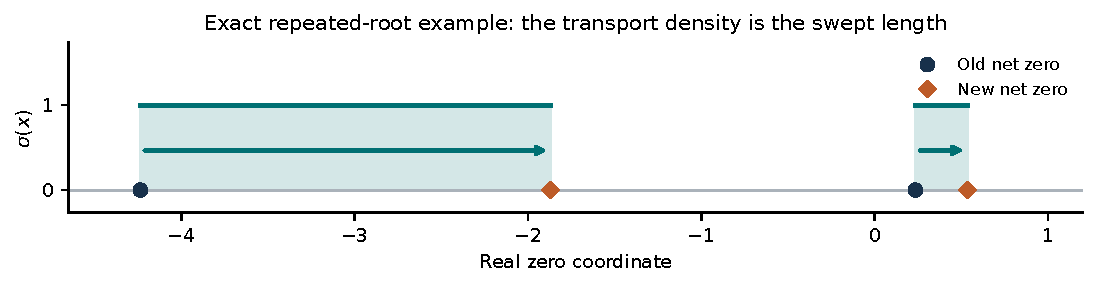
\includegraphics[width=\linewidth]{figures/finite_transport.pdf}
\caption{Exact finite example after common zero factors are cancelled
with their multiplicities.  The shaded area is total displacement.
The endpoints shown are the exact radicals given in the text.}
\end{figure}

For both polynomial examples, the script compares the exact determinant
phase with the sum of arctangent integrals over the moving intervals
and with numerical quadrature.  The largest recorded numerical
discrepancy was below $3\times10^{-66}$ at 180-digit working precision.
Exact symbolic identities and floating-point comparisons are separately
labelled in \texttt{data/verification.json}.

\subsection{Dirichlet and electrical transform checks}

For the ordinary construction, use the path Laplacian
\[
 A=\begin{pmatrix}1&-1&0\\-1&2&-1\\0&-1&1\end{pmatrix},
 \qquad B=(e_1-e_3)(e_1-e_3)^{\mathsf T},
\]
and inputs of conductors $1,3,4$, respectively.  The conductor-one input
is zeta; the other two are the real primitive characters.  Their
logarithmic derivatives at $iy$ are evaluated on the positive real
half-plane using the functional equation, the digamma function, and
finite Dirichlet sums.  The elementary tail bounds, for $s>1$, are
\[
 \left|\sum_{n>N}\frac{\chi(n)}{n^s}\right|
 \le\frac{N^{1-s}}{s-1},\quad
 \left|\sum_{n>N}\frac{\chi(n)\log n}{n^s}\right|
 \le N^{1-s}\left(\frac{\log N}{s-1}+\frac1{(s-1)^2}\right).
\]
The script records these truncation estimates and compares three-term
and 96-term matrix expansions.  The latter is used only in a region
where the matrix logarithm power series converges.

The ordinary normalized column below is
\[
 R_{\rm ord}(y)=\frac{\log y}{2\operatorname{tr}B}
                \operatorname{Im}\mathcal L_{A,B}(iy),
\]
whose limit is one.  For the squared construction, use three zeta inputs
on the same path and triangle, put $R=y^2$, and write $r(-R)$ for the
spanning-tree-normalized ratio in \eqref{eq:squared-stieltjes}.
The second normalization is
$R_{\rm sq}(y)=12\sqrt R\log r(-R)/\log R$, also with limit one.

\begin{center}
\begin{tabular}{rrr}
\toprule
$\log y$ & $R_{\rm ord}(y)$ & $R_{\rm sq}(y)$\\
\midrule
5   &0.64919196&0.63942986\\
10  &0.93622765&0.81627860\\
20  &1.01318185&0.90810615\\
50  &1.01626695&0.96324246\\
100 &1.00983903&0.98162123\\
200 &1.00532818&0.99081061\\
\bottomrule
\end{tabular}
\end{center}

\begin{figure}[ht]
\centering
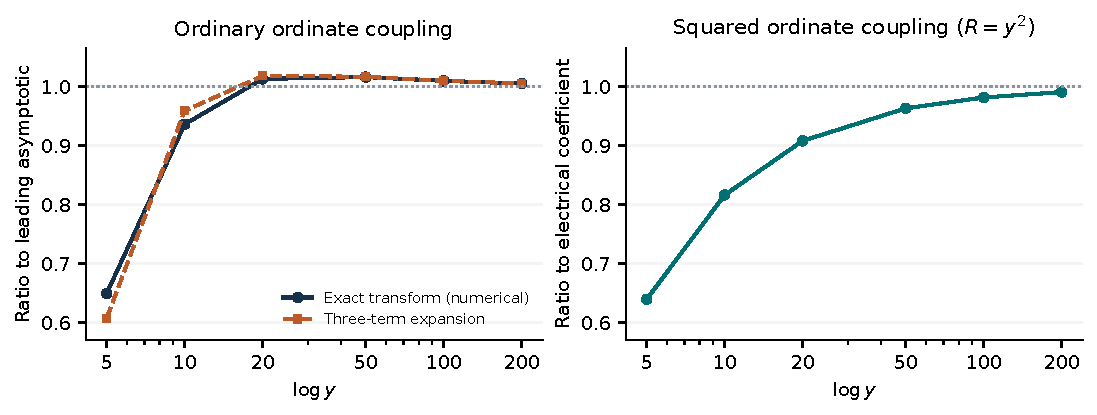
\includegraphics[width=\linewidth]{figures/transform_convergence.pdf}
\caption{Floating-point diagnostics of the exact transform formulas.
Each ratio tends to one.  These plots evaluate finite determinants and
positive-real Dirichlet expressions; they do not sum or certify an
infinite set of numerical zeros.}
\end{figure}

\subsection{What has and has not been checked}

The proofs of the transport constants, Poisson limit, moving-band local
law, and electrical companion were independently re-derived within this
research session.  The separate audit notes record the branch choice,
tail control, multiple-zero treatment, and squared-variable restriction.
They are mathematical review notes, not external peer review or formal
proof certificates.

The Python assertions passed.  Rational identities and root-isolation
checks are exact; mpmath output is not rigorously rounded.  Analytic
truncation bounds are supplied, but their decimal evaluations are not
interval certificates.  The unsmoothed and arbitrarily shrinking-band
claims rest on their proofs, not on the numerical figures.  No fresh
Lean build of the upstream theorem and no Lean formalization of the new
results is claimed.

The conductors, number of inputs, and graph matrices are fixed in the
matrix theorems.  The scalar theorem explicitly allows its tested value
interval to vary with $T$.  The squared theorem requires even inputs;
a single complex-character completion generally is not even.  No
consequence about all automorphic $L$-functions, new Euler products,
simple zeta zeros, or individual zero spacings is asserted.

\subsection{Reproducing the packet}

From the archive's top directory, run
\begin{verbatim}
python3 code/verify_transport.py
python3 code/make_figures.py
latexmk -pdf -interaction=nonstopmode paper.tex
\end{verbatim}
The first command regenerates the recorded JSON.  The second regenerates
the vector figures and PNG previews.  The third compiles this report
with a standard TeX Live installation.  A portable Python build helper
is also included for installations that have TeX sources but no generated
format or font map.  All source sections and figure assets needed to
compile the supplied document are in the archive.

For later formalization, the useful separation is: real canonical
products and strict half-plane sign; finite Hermitian inertia and matrix
logarithms; the positive Poisson rescaling lemma; and the Dirichlet
radial asymptotic.  The moving-window theorem then requires only scalar
integration and that rescaling lemma, while the electrical companion
adds the two-root forest identity and a positive Stieltjes Tauberian step.
This is a dependency plan, not a claimed executable Lean proof.

\begin{thebibliography}{99}
\bibitem{upstream}
L. Sernau and collaborators, \emph{GRH for Dirichlet $L$-functions, in Lean 4}.
Pinned commit \texttt{72fead102f663d5c7a407964a13dc0cf9d977207}, November 25, 2026.
\href{https://github.com/lsernau/grh-lean/tree/72fead102f663d5c7a407964a13dc0cf9d977207}{Repository and pinned source}.
Central paths: \texttt{grh-compact/src/Statements.lean},
\texttt{src/New/Main.lean}, and \texttt{src/New/Endgame/}.

\bibitem{sutherland}
A. Sutherland, \emph{Verification files for the shorter Lean proof of RH and GRH},
November 2026. \url{https://math.mit.edu/~drew/shortgrh/}.
This report cites the published check record; it does not claim a fresh replay.

\bibitem{wikipedia}
Wikipedia contributors, \emph{Riemann hypothesis}, page inspected November 26, 2026.
\url{https://en.wikipedia.org/wiki/Riemann_hypothesis}.
Used for the requested historical/status comparison; formal scope comes from
the primary Lean statements.

\bibitem{proveit}
V. Reshetnikov, \emph{ProveIt: Analysis/GeneralizedRiemannHypothesis},
commit \texttt{041d8032541746f2ac2e686fbe437f8092771670}.
\href{https://github.com/VladimirReshetnikov/ProveIt/tree/041d8032541746f2ac2e686fbe437f8092771670/Analysis/GeneralizedRiemannHypothesis}{Pinned research tree}.
The README distinguishes imported research from checked formalization.

\bibitem{priorgraph}
\emph{Graph-coupled zeros}, ProveIt research packet,
\texttt{graph\_coupled\_zeros\_2026-11-26.zip}, November 26, 2026.
\href{https://github.com/VladimirReshetnikov/ProveIt/blob/041d8032541746f2ac2e686fbe437f8092771670/Analysis/GeneralizedRiemannHypothesis/docs/incoming/graph_coupled_zeros_2026-11-26.zip}{Pinned archive}.
See \texttt{sections/electrical.tex}, \texttt{sections/entire.tex}, and the
open questions in \texttt{sections/verification.tex}.

\bibitem{dlmfdirichlet}
NIST Digital Library of Mathematical Functions, \S25.15,
\emph{Dirichlet $L$-functions}; and \S5.11, asymptotic expansions of gamma functions.
\url{https://dlmf.nist.gov/25.15}; \url{https://dlmf.nist.gov/5.11}.

\bibitem{reiffenstein}
J. Reiffenstein, \emph{Higher-order interlacing for matrix-valued meromorphic
Herglotz functions}, J. Math. Anal. Appl. \textbf{514} (2022), 126260.
\url{https://arxiv.org/abs/2108.10746}.

\bibitem{bgn}
J. Behrndt, F. Gesztesy, and S. Nakamura, \emph{Spectral shift functions and
Dirichlet-to-Neumann maps}, Math. Ann. \textbf{371} (2018), 1255--1300.
\url{https://arxiv.org/abs/1609.08292};
\href{https://doi.org/10.1007/s00208-017-1593-4}{DOI: 10.1007/s00208-017-1593-4}.

\bibitem{langerworacek}
M. Langer and H. Woracek, \emph{Karamata's theorem for regularised Cauchy
transforms}, Proc. Roy. Soc. Edinburgh Sect. A \textbf{155} (2025), 1431--1491.
\url{https://arxiv.org/abs/2307.12249}.
See Theorem 4.7 and Appendix Theorem A.7, Remark A.8.

\bibitem{aizenmanwarzel}
M. Aizenman and S. Warzel, \emph{On the ubiquity of the Cauchy distribution
in spectral problems}, Probab. Theory Related Fields \textbf{163} (2015), 61--87.
\url{https://arxiv.org/abs/1312.7769}.

\bibitem{sodin}
S. Sodin, \emph{On the critical points of random matrix characteristic
polynomials and of the Riemann $\xi$-function}, Q. J. Math. \textbf{69}
(2018), 183--210. \url{https://arxiv.org/abs/1611.10037}.
See \S3.4.5, equation (55), for the scalar weak Cauchy law.

\bibitem{najnudel}
J. Najnudel and A. Nikeghbali, \emph{Cauchy laws for zeta logarithmic
derivatives and stationary Stieltjes transforms}, arXiv:2609.15862v1,
September 14, 2026. \url{https://arxiv.org/abs/2609.15862}.
See Theorem 1.1 and the paragraph following equation (1.4).

\bibitem{lagarias}
J. C. Lagarias, \emph{Zero spacing distributions for differenced $L$-functions},
Acta Arith. \textbf{120} (2005), 159--184.
\url{https://arxiv.org/abs/math/0601653}.

\bibitem{farmergonek}
D. W. Farmer, S. M. Gonek, and Y. Lee, \emph{Pair correlation of the zeros
of the derivative of the Riemann $\xi$-function}, J. London Math. Soc.
\textbf{90} (2014), 241--269.
\url{https://arxiv.org/abs/0803.0425}.
\end{thebibliography}

\end{document}
